\section{Introduction}

\subsection{Microelectronic Economics}
\begin{itemize}
\item \textbf{Fixed Costs}: Design
\item \textbf{Variable Costs}: Energy for manufacturing, material needed
\end{itemize}
The higher the integration level, the better and cheaper the final product, true for high-volume production. In fact volume recaptures manufacturing and designs cost.
\bigskip \\
For applications that do not enjoy high-volume (ASICs), other factors matter: reduction of design time (and cost) and quality of the design.
\bigskip \\
\textbf{Variability}: variation of the geometry of transistor that introduce error about speed because \textit{lithography} is not so precise and do not allow to create a good channel in the transistors.

\subsection{CAD}
\textbf{CAD} (Computer-Aided Design) allow to:
\begin{itemize}
\item Reduces design time
\item Multi-objective optimization (area, speed, power)
\item Large scale design management
\end{itemize}
CAD tools reduce time to market, reducing the \textit{fixed cost}. Moreover you can also reduce the \textit{variable cost} optimizing the area and using less silicon.

\subsection{Integrated Circuit Design Styles}
\begin{figure}[H]
	\centering
	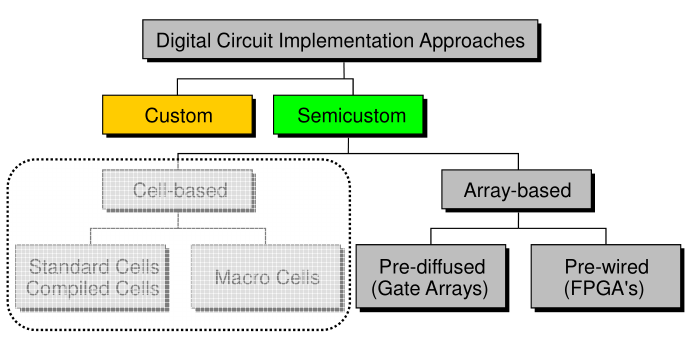
\includegraphics[height=90 mm]{./Cap1/Images/Image01.png}
	\caption[Optional caption]{Integrated Circuit Design Styles}
	\label{fig:ICDS}
\end{figure}
The \textbf{custom} approach (design \textit{by hand}):
\begin{itemize}
\item Functional and physical design are hand-crafted operations
\item Extensive effort (and cost) to optimize each feature
\item Typical of \textit{critical portions} of high-performance designs
\end{itemize}
The \textbf{Semi-custom} approaches
\begin{itemize}
\item Limited number of circuits primitives that allows designers to leverage “optimized” primitives and focus on their \textit{interconnection}
\item Semi-custom design are the big majority of digital design
\end{itemize}
Type of \textbf{Semi-custom} approaches:
\begin{itemize}
\item \textbf{Cell-based}: use  standard cells  or  macrocells  (larger functions)
\begin{itemize}
\item \textbf{Standard cells}: Designed once and highly optimized, stored into a library
\item  \textbf{Macrocells}: Primitives generated by  module generators, ynthesized layout thanks to predefined structures (SRAMs, ROMs)
\end{itemize}
\item \textbf{Array-based}:  Exploit the use of a matrix of uncommitted components which are eventually personalized and connected
\begin{itemize}
\item \textbf{Re-diffused arrays}: Personalization by metalization/contacts (MPGAs).
\item \textbf{Pre-wired arrays}: Personalization on the field (FPGAs).
\end{itemize}
\end{itemize}

\subsection{Microelectronic Design}
Three major tasks (repeated at different \textit{Abstraction levels}):
\begin{itemize}
\item \textbf{Conceptualization and modeling} (Description): Hardware Description Languages (HDL)
\item \textbf{Synthesis and optimization}: Create the structure
\item \textbf{Validation}: Check for correctness
\end{itemize}
\textbf{Models} can be classified in terms of
\begin{itemize}
\item \textit{Abstraction levels}
\begin{itemize}
\item \textbf{Architectural-level} (or RT-level): Operations implemented by
resources.
\item \textbf{Logic-level}: Logic functions implemented by gates.
\item \textbf{Geometrical-level} (or Circuit-level): Circuit implemented by electronic device
\end{itemize}
\item \textit{Views}
\begin{itemize}
\item \textbf{Behavioral} view: Abstract function.
\item \textbf{Structural} view: An interconnection of parts.
\item \textbf{Physical} view: Physical objects with size and positions.
\end{itemize}
\end{itemize}
\begin{figure}[H]
	\centering
	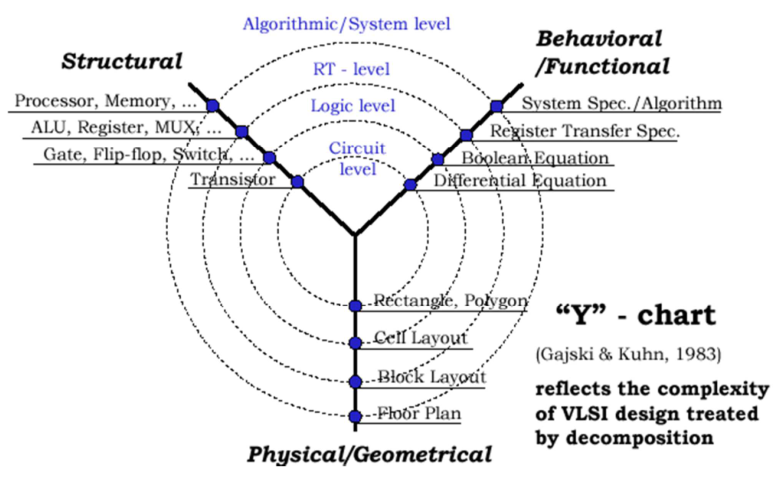
\includegraphics[height=90 mm]{./Cap1/Images/Image02.png}
	\caption[Optional caption]{Y chart}
	\label{fig:Ychart}
\end{figure}
In the Figure \ref{fig:Ychart} the axis represent the \textit{Abstraction levels}, the circles the \textit{Views}.\\
It shows the same \textit{Abstraction levels} at different \textit{Views} and vice versa.\\
The \textbf{synthesis} is the switching from Behavioural to Structural at different \textit{Abstraction levels} and Optimization.\\
Objectives of the Optimization:
\begin{itemize}
\item Area
\item Timing (Performance)
\item Energy consumption
\end{itemize}
Optimization has multiple objectives, it is a trade off.
\begin{figure}[H]
	\centering
	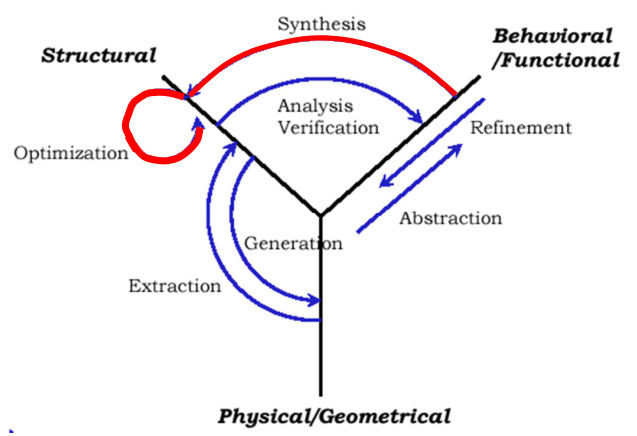
\includegraphics[height=70 mm]{./Cap1/Images/Image03.png}
	\caption[Optional caption]{Synthesis and Optimization}
	\label{fig:SynthOpt}
\end{figure}
\begin{flushleft}
	The \textbf{design} is the repetition of
\end{flushleft}
\begin{enumerate}
\item Modelling
\item Synthesis \& Optimization
\item Validation
\end{enumerate}
for each level: RTL, LOGIC, PHYSICAL.

\subsection{Design space}
The Design Space is where a dimension is a variable. The different feasible structural implementations of a circuit define its design space. The design space is a finite set of design points. Combined optimization of area (minimization) and performance (maximization) can be abstracted by representing the feasible structural implementations of a design into a design space.
\bigskip \\
\textbf{Optimization}: search an implementation that optimizes all
objectives.
\bigskip \\
A  point of the design space is called a  \textbf{Pareto point} if there is no other point (in the design space) with at least an inferior objective, all others being inferior or equal. A Pareto point corresponds to a global optimum in a monodimensional design evaluation space.\\ 
The image of the Pareto points in the design evaluation space is the set of the optimal  trade-off  points. Their interpolation yields a  trade-off curve  or  surface.
\begin{figure}[H]
	\centering
	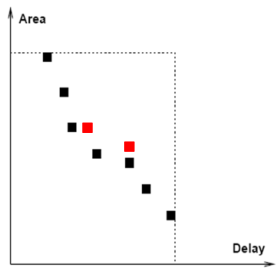
\includegraphics[height=50 mm]{./Cap1/Images/Image04.png}
	\caption[Optional caption]{Pareto Points}
	\label{fig:Pareto}
\end{figure}
\begin{flushleft}
	In the Figure \ref{fig:Pareto} the black points are the Pareto points.
\end{flushleft}

\subsection{General approaches to optimization}
Circuit optimization involves multiple objective functions. The optimization problem is difficult to solve, due to the discontinuous nature of the objective functions and to the discrete nature of the design space, i.e., of the set of feasible circuit implementations. In general, Pareto points  are  solutions to constrained optimization problems.\\
Consider, for example, \textit{logic-level} models. Then the following two problems are of interest:
\begin{itemize}
\item Minimize the circuit  \textit{area}  under  \textit{delay} constraints
\item Minimize the circuit  \textit{delay}  under  \textit{area} constraints
\end{itemize}
Unfortunately, due to the difficulty of the optimization problems, only approximations to the Pareto points can be computed.\\
Consider next \textit{architectural-level} models of synchronous circuits. Pareto points are solutions to the following problems, for different values of the \textbf{cycle-time}:
\begin{itemize}
\item Minimize the circuit \textit{area} under \textit{latency} constraints
\item Minimize the circuit \textit{latency} under \textit{area} constraints
\end{itemize}
These two problems are often referred to as \textit{scheduling problems}.
